%% Fig 17: T1 Spearman correlation heatmap (model x grid)
%% Diverging colormap: blue (negative) - white - orange (positive)
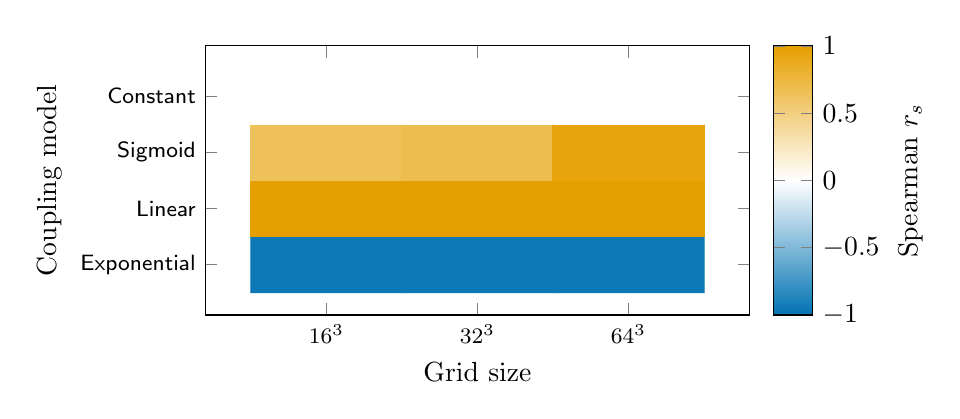
\begin{tikzpicture}
\begin{axis}[
  width=0.7\textwidth,
  height=5cm,
  view={0}{90},
  colormap={OIdiverg}{
    rgb255=(0,114,178)
    rgb255=(255,255,255)
    rgb255=(230,159,0)
  },
  colorbar,
  colorbar style={
    ylabel={Spearman $r_s$},
    ytick={-1,-0.5,0,0.5,1},
  },
  point meta min=-1,
  point meta max=1,
  xlabel={Grid size},
  ylabel={Coupling model},
  xtick={0,1,2},
  xticklabels={$16^3$, $32^3$, $64^3$},
  ytick={0,1,2,3},
  yticklabels={Exponential, Linear, Sigmoid, Constant},
  y tick label style={font=\sffamily\footnotesize},
  x tick label style={font=\sffamily\footnotesize},
]
  %% Matrix data: (grid_idx, model_idx) [r_s value]
  %% Exp: -0.952 at all grids
  %% Linear: +1.000 at all grids
  %% Sigmoid: +0.643, +0.690, +0.952
  %% Constant: 0.000 at all grids
  \addplot[matrix plot*, mesh/cols=3, mesh/rows=4, point meta=explicit]
    coordinates {
      (0,0) [-0.952]  (1,0) [-0.952]  (2,0) [-0.952]
      (0,1) [1.000]   (1,1) [1.000]   (2,1) [1.000]
      (0,2) [0.643]   (1,2) [0.690]   (2,2) [0.952]
      (0,3) [0.000]   (1,3) [0.000]   (2,3) [0.000]
    };
\end{axis}
\end{tikzpicture}
